Para la solución del sistema lineal $Ax = b$ con:\\
\begin{gather*}
A = 
\begin{bmatrix}
       1   &     2 \\
       2   &     3 \\
\end{bmatrix},
b = 
\begin{bmatrix}
    3 \\
    5 \\
\end{bmatrix}
\end{gather*}
Considere el siguiente método iterativo
\begin{gather*}
x^{(k+1)} = B(\theta)x^{(k)} + g(\theta), \>\>\>\> k \geq 0, \>\>\>\> con\>x^{(0)}\>dado,\\
Donde\>\theta\>es\>un\>par\acute ametro\>real\>y \\
B(\theta) = \frac{1}{4}\begin{bmatrix}
       2\theta^2 + 2\theta + 1   &     -2\theta^2 + 2\theta + 1 \\
       -2\theta^2 + 2\theta + 1   &     2\theta^2 + 2\theta + 1 \\
\end{bmatrix},\>\>
g(\theta)= \begin{bmatrix}
    \frac{1}{2} -\theta \\
    \frac{1}{2} -\theta \\
\end{bmatrix}
\end{gather*}
Verifique que el método es consistente $\forall\theta\in {\rm I\!R}$. Luego, determine los valores de $\theta$ para el cual el método es convergente y calcule el valor óptimo de $\theta$ (ejm., el valor del parámetro para el cual la tasa de convergencia es máxima).\\\\

\textbf{\underline{Solución:}}

\begin{itemize}
\item [$i)$] Consistencia del método\\

Analizando para la convergencia $X^{(k+1)}=X^k$, según lo cual:\\
$$x^{(k)} = B(\theta)x^{(k)} + g(\theta)$$
$$g(\theta) =  (I-B(\theta))x^{(k)}$$
$$g(\theta) = (I-B(\theta))A^{-1}.b $$
Para comprobar la consistencia del método será necesario corroborar que igualdad anterior cumple $\forall \theta$.
Para ello solamente es necesario reemplazar en los valores dados inicialmente, obteniendo:
\begin{gather*}
	\begin{bmatrix}
    	\frac{1}{2} -\theta \\
    	\frac{1}{2} -\theta 
	\end{bmatrix} = (
   \begin{bmatrix}
       1   &     0 \\
       0   &     1 \end{bmatrix} - 
       \frac{1}{4}
   \begin{bmatrix}
       2\theta^2 + 2\theta + 1   &     -2\theta^2 + 2\theta + 1 \\
       -2\theta^2 + 2\theta + 1   &     2\theta^2 + 2\theta + 1 \\
	\end{bmatrix})
    \begin{bmatrix}
       1   &     2 \\
       2   &     3 \\
	\end{bmatrix}^{-1}
    \begin{bmatrix}
      3 \\
      5 \\
	\end{bmatrix}
    \\
    \begin{bmatrix}
    	\frac{1}{2} -\theta \\
    	\frac{1}{2} -\theta 
	\end{bmatrix} = 
   	\begin{bmatrix}
       -\frac{1}{2}\theta^2 - \frac{1}{2}\theta + \frac{3}{4} & \frac{1}{2}\theta^2 - \frac{1}{2}\theta - \frac{1}{4} \\
       \frac{1}{2}\theta^2 - \frac{1}{2}\theta - \frac{1}{4} & -\frac{1}{2}\theta^2 - \frac{1}{2}\theta + \frac{3}{4}
	\end{bmatrix}
    \begin{bmatrix}
       -3   &     2 \\
        2   &    -1 \\
	\end{bmatrix}
    \begin{bmatrix}
      3 \\
      5 \\
	\end{bmatrix}
    \\
    \begin{bmatrix}
    	\frac{1}{2} -\theta \\
    	\frac{1}{2} -\theta 
	\end{bmatrix} = 
   	\begin{bmatrix}
       -\frac{1}{2}\theta^2 - \frac{1}{2}\theta + \frac{3}{4} & \frac{1}{2}\theta^2 - \frac{1}{2}\theta - \frac{1}{4} \\
       \frac{1}{2}\theta^2 - \frac{1}{2}\theta - \frac{1}{4} & -\frac{1}{2}\theta^2 - \frac{1}{2}\theta + \frac{3}{4}
	\end{bmatrix}
    \begin{bmatrix}
      1 \\
      1 \\
	\end{bmatrix}
\end{gather*}
Operando, se tiene:
\begin{gather*}
	\begin{bmatrix}
    	\frac{1}{2} -\theta \\
    	\frac{1}{2} -\theta 
	\end{bmatrix} = 
   	\begin{bmatrix}
       (-\frac{1}{2}\theta^2 - \frac{1}{2}\theta + \frac{3}{4}) + (\frac{1}{2}\theta^2 - \frac{1}{2}\theta - \frac{1}{4})\\
       (\frac{1}{2}\theta^2 - \frac{1}{2}\theta - \frac{1}{4}) + (-\frac{1}{2}\theta^2 - \frac{1}{2}\theta + \frac{3}{4})
	\end{bmatrix}\\
	\begin{bmatrix}
    	\frac{1}{2} -\theta \\
    	\frac{1}{2} -\theta 
	\end{bmatrix} = 
	\begin{bmatrix}
       -\frac{2}{2}\theta + \frac{2}{4}\\
       -\frac{2}{2}\theta + \frac{2}{4}\\
	\end{bmatrix}\\
	\begin{bmatrix}
    	\frac{1}{2} -\theta \\
    	\frac{1}{2} -\theta 
	\end{bmatrix} = 
	\begin{bmatrix}
    	\frac{1}{2} -\theta \\
    	\frac{1}{2} -\theta 
	\end{bmatrix}
\end{gather*}
Por lo tanto, el método iterativo es consistente $\forall\theta\in {\rm I\!R}$.\\\\


\item [$ii)$]  Valores de $\theta$ para el cual el método es convergente:\\

Para la determinación de la convergencia del método se requiere calcular el radio espectral de la matriz $B$, $\rho(B)$.  Segun esto procedemos al cálculo de los auovalores mediante $det(B - \lambda I) = 0$:\\
\begin{gather*}
\begin{vmatrix}
       \frac{1}{4}(2\theta^2 + 2\theta + 1) - \lambda  &     \frac{1}{4}(-2\theta^2 + 2\theta + 1) \\
       \frac{1}{4}(-2\theta^2 + 2\theta + 1)   &     \frac{1}{4}(2\theta^2 + 2\theta + 1)  - \lambda \\ 
\end{vmatrix} = 0\\
    (\frac{1}{16}(2\theta^2 + 2\theta + 1) - \lambda)((2\theta^2 + 2\theta + 1)  - \lambda) - \frac{1}{16}(-2\theta^2 + 2\theta + 1)(-2\theta^2 + 2\theta + 1) = 0\\
    \frac{1}{16}(2\theta^2 + 2\theta + 1)^2 - \frac{2}{4}(2\theta^2 + 2\theta + 1)\lambda +  \lambda^2 - \frac{1}{16}(-2\theta^2 + 2\theta + 1)^2 = 0\\
    (\frac{1}{16}((2\theta^2+2\theta + 1)^2 - (-2\theta^2+2\theta + 1)^2) - \frac{1}{2}(2\theta^2 + 2\theta + 1)\lambda +  \lambda^2 = 0\\
    \frac{1}{16}.4(2\theta + 1)(2\theta^2) - \frac{1}{2}(2\theta^2 + 2\theta + 1)\lambda +  \lambda^2 = 0\\
    \frac{1}{4}(2\theta + 1)(2\theta^2) - \frac{1}{2}(2\theta^2 + 2\theta + 1)\lambda +  \lambda^2 = 0
\end{gather*}
Factorizando:
\begin{gather*}
    (\lambda - \theta^2)(\lambda - \frac{1}{2}(2\theta + 1)) = 0\\
    \lambda = \theta^2\>\>\>\> \vee \>\>\>\> \lambda = \frac{1}{2}(2\theta + 1)
\end{gather*}
El resultado que se obtuvo es el valor de $\lambda$ en función al valor de $\theta$:
\begin{figure}[H]
  \centering
  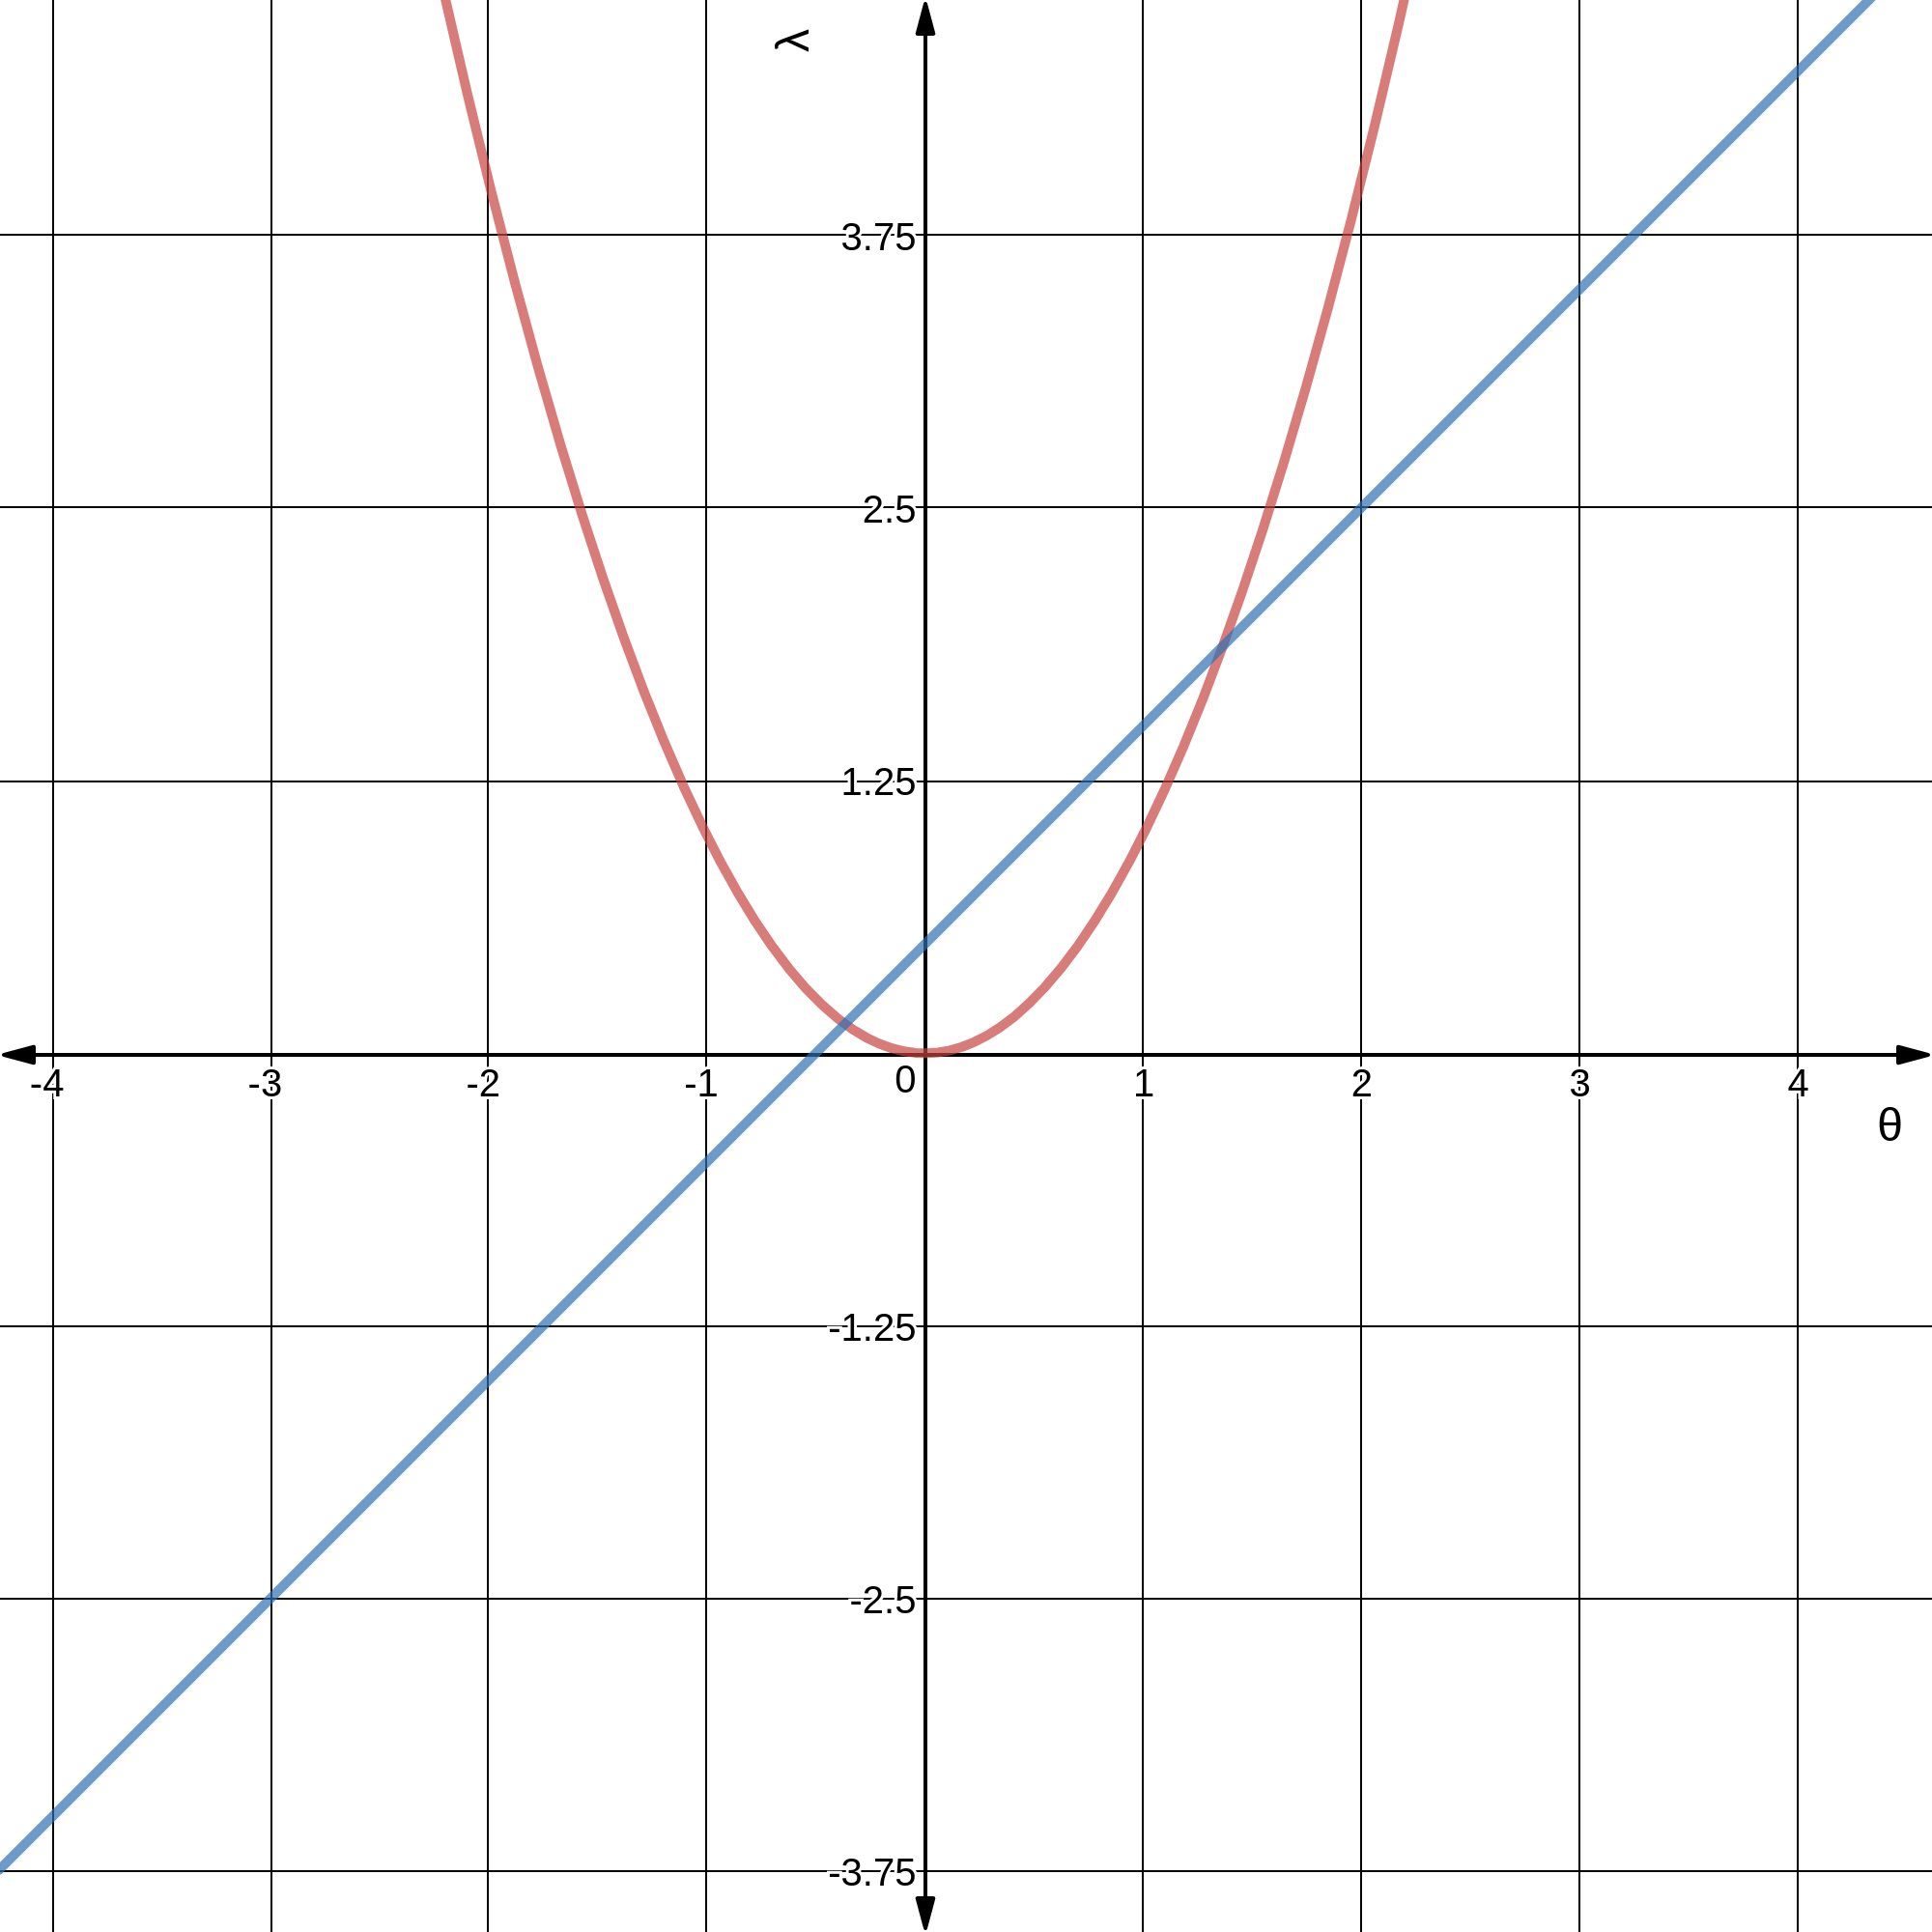
\includegraphics[width=250px]{images/graph_q5.png}
  \caption{Gr\'afico de la función.}
  \label{fig:graph5}
\end{figure}

Debido a que $\rho$ es el máximo autovalor de $B$, entonces toma los siguentes valores en función a $\theta$:

\[   
\rho(B) = 
     \begin{cases}
       \theta^2 & \theta\leq\frac{1-\sqrt{3}}{2}\\
       \frac{1}{2}(2\theta + 1) & \frac{1-\sqrt{3}}{2}<\theta
     \end{cases}
\]

Para que el método sea convergente, se debe cumplir que $\rho(B) < 1$, por lo que el gráfico de $\rho(B)$ en función de $\theta$ será:
\begin{gather*}
    \theta^2 < 1\>\>\>\wedge\>\>\> \frac{1}{2}(2\theta + 1) < 1\\
    -1 < \theta < 1\>\>\>\wedge\>\>\> \theta < \frac{1}{2}\\
    -1 < \theta < \frac{1}{2}
\end{gather*}

\begin{figure}[H]
  \centering
  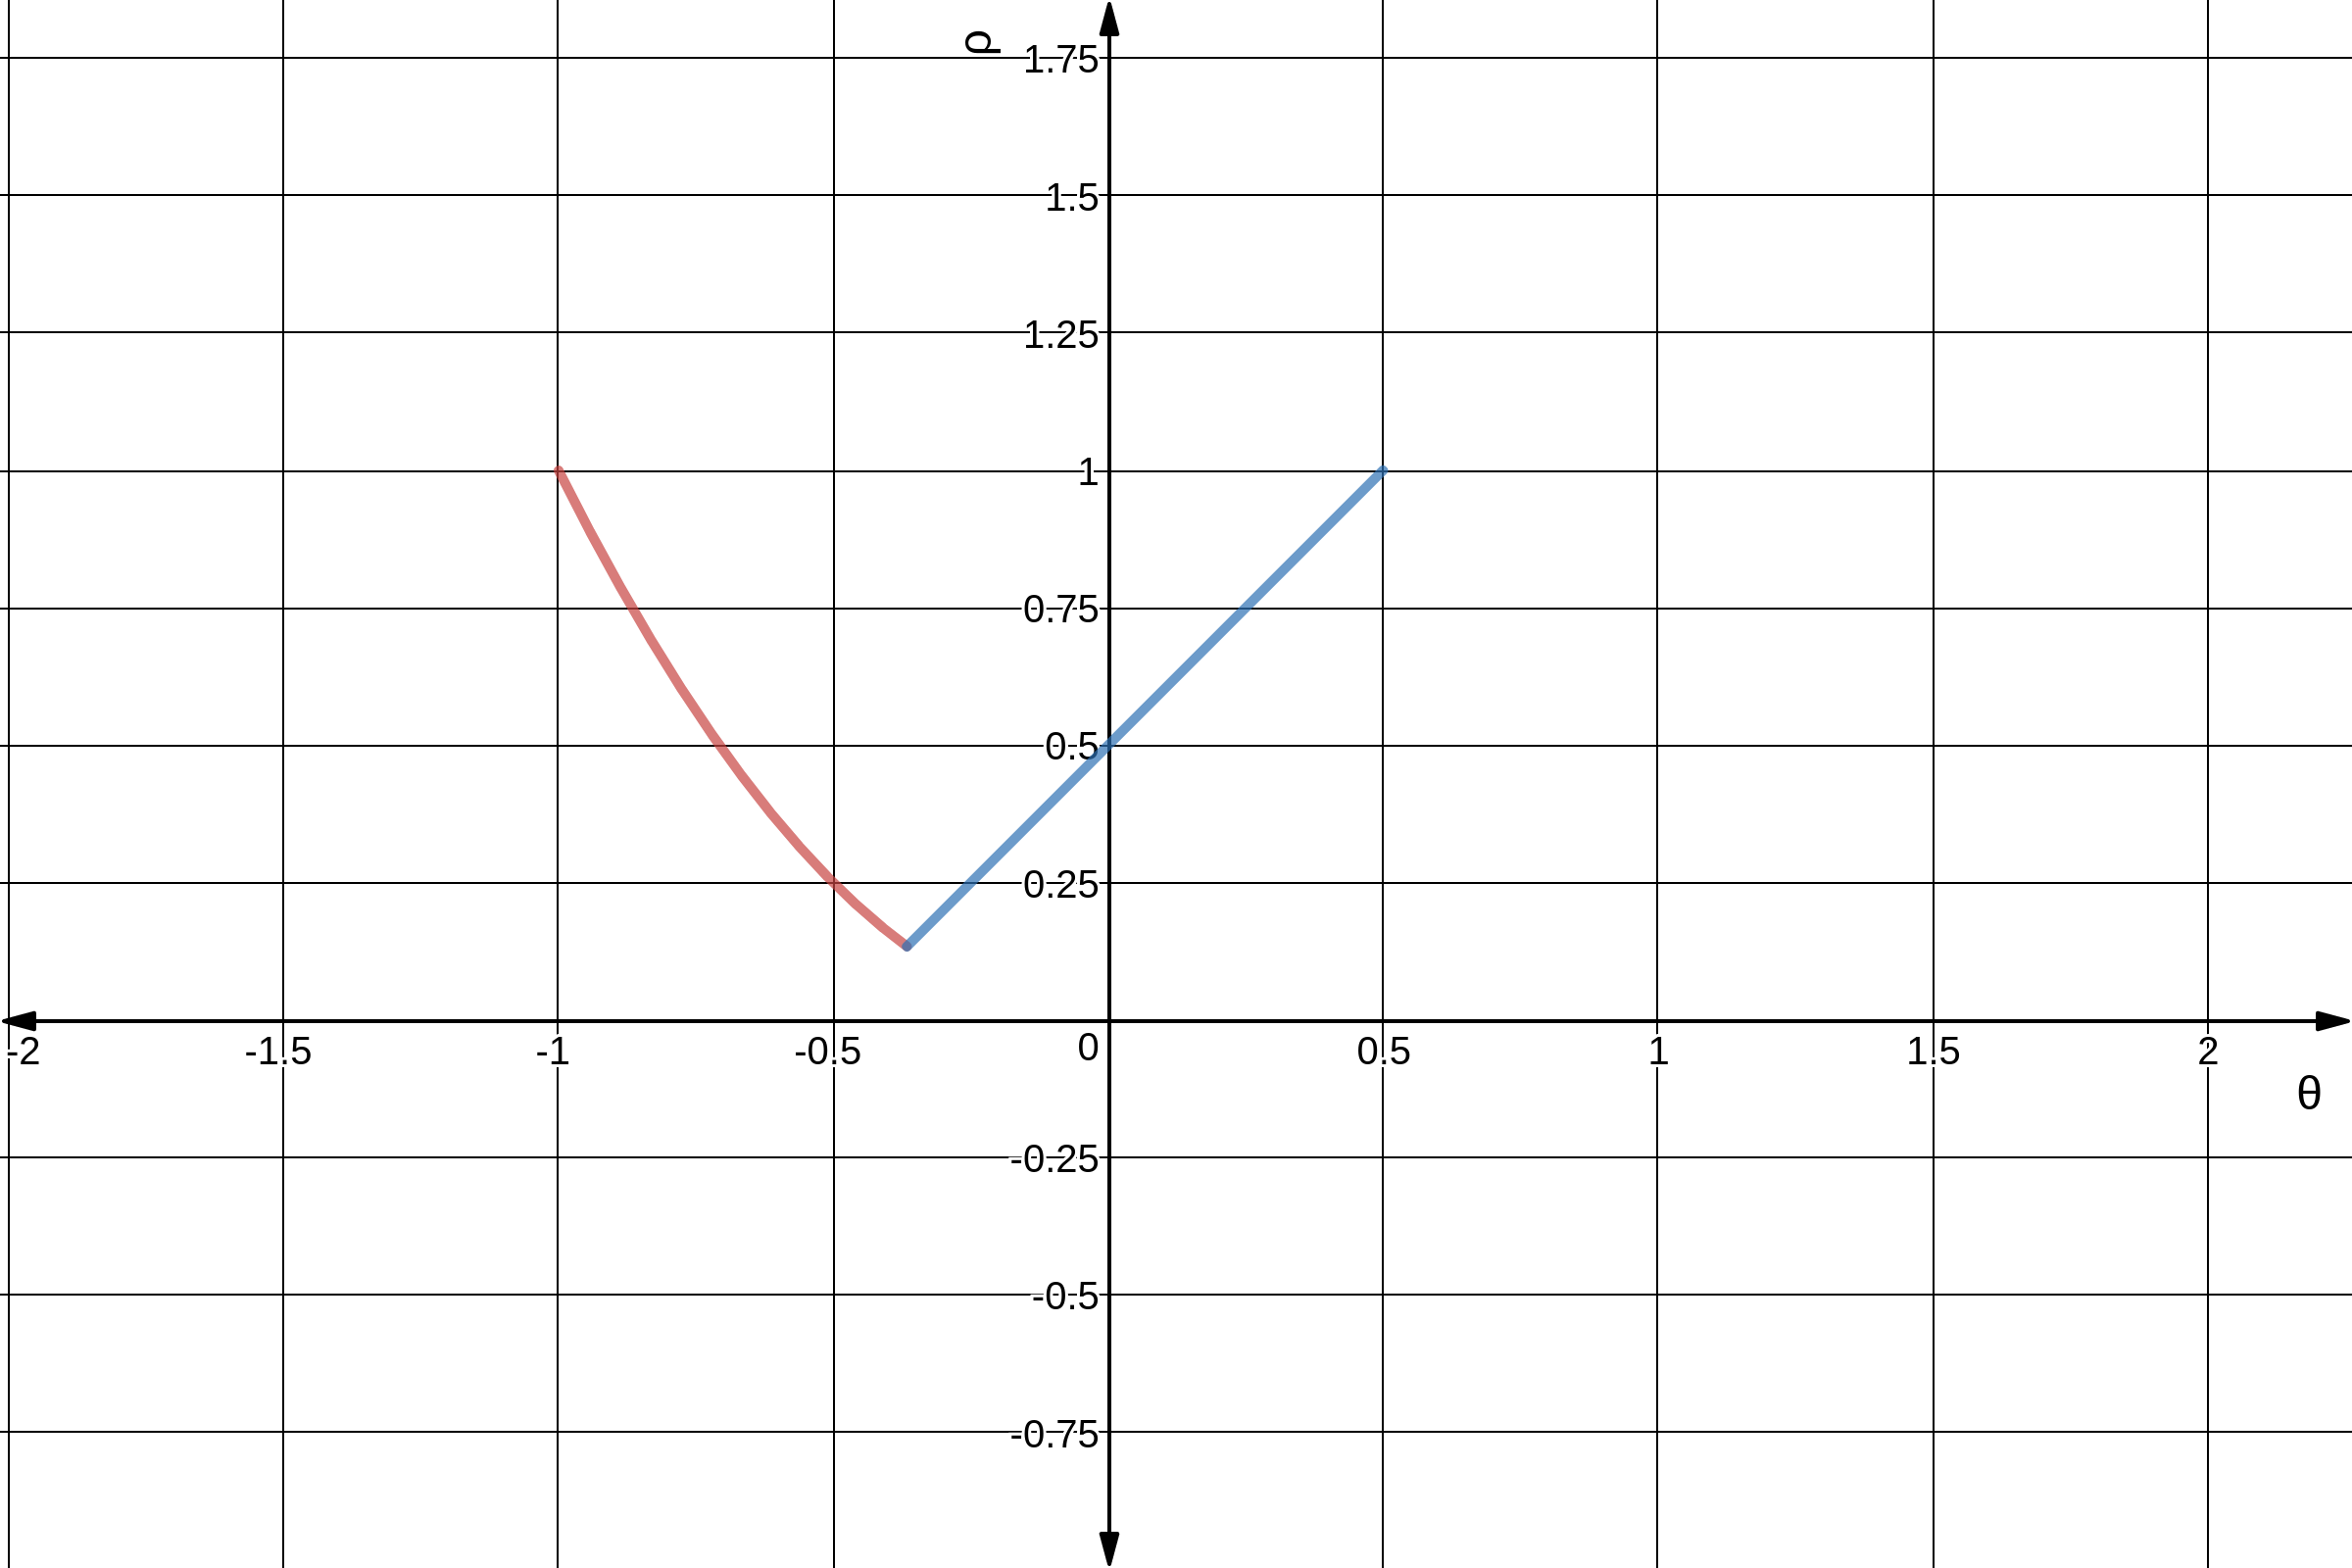
\includegraphics[width=250px]{images/graph2_q5.png}
  \caption{Gr\'afico de $\rho(B)$ en funci\'on a $\theta$.}
  \label{fig:graph6}
\end{figure}

Como se puede apreciar, el método es convergente si $-1 < \theta < \frac{1}{2}$

$iii)$ Valor óptimo de $\theta$:\\
Partiendo del intervalo de los valores de $\rho(B)$:
\begin{gather*}
    \rho(B)(\theta = \frac{1-\sqrt{3}}{2}) \leq \rho(B) < 1
\end{gather*}
Aplicaremos $-log$ a todos los miembros, ya que $-log(\rho(B))$ es la tasa de convergencia asimptótica:
\begin{gather*}
    -log(\rho(B)(\theta = \frac{1-\sqrt{3}}{2})) \leq -\log(\rho(B)) < -log(1)\\
    log(\rho(B)(\theta = \frac{1-\sqrt{3}}{2})) \geq \log(\rho(B)) > log(1)
\end{gather*}

Por lo tanto el valor óptimo de $\theta$ (el valor para el cual la tasa de convergencia es máxima) es:
\begin{gather*}
    \theta = \frac{1-\sqrt{3}}{2}
\end{gather*}

\end{itemize}